\section{Modelling mathematics}

In order to program a neural network, it is necessary to first enumerate the
differential equations that describe constituent neurons of a network, and the
rules that govern the interactions between them. A neuron state at a given time
is typically defined by a collection of differential equations, where spikes
occur as a response to changes in this state \autocite{brette_simulation_2007}.
In the following section I will define and justify the behaviour of these
neurons.

\subsection{Leaky Integrate and Fire}

The simplest approximation of a spiking neuron that retains the chemical
behaviour of a biological action potential are Leaky Integrate and Fire (LIF)
neurons. As any neuron is, in effect, a signal processing unit, they can be
modelled as a circuit.

\begin{figure}[h!]
    \begin{subfigure}{.5\textwidth}
        \centering
        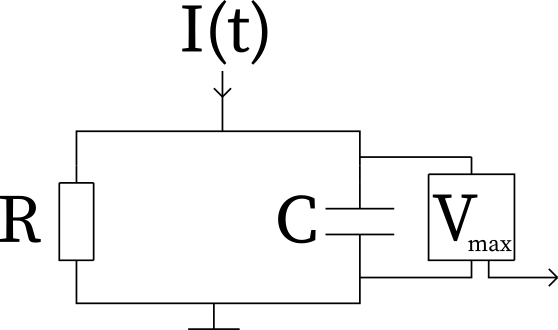
\includegraphics[width=.9\linewidth]{figures/images/LIFCircuit1.png}
        \caption{IF model}
        \label{fig:LIFSchemA}
    \end{subfigure}%
    \begin{subfigure}{.5\textwidth}
        \centering
        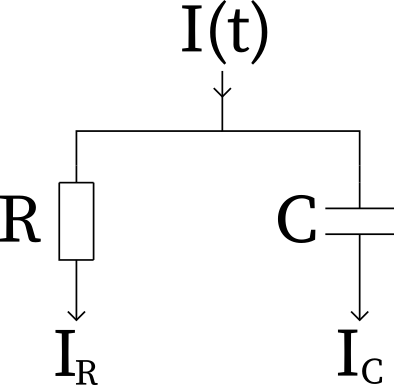
\includegraphics[width=.7\linewidth]{figures/images/LIFCircuit2.png}
        \caption{IF Currents}
        \label{fig:LIFSchemB}
    \end{subfigure}
    \DoubleCaption{Schematics of an Integrate and Fire model}{\small{Redrawn and
            adapted from \cite{gerstner_spiking_2002}}}
    \label{fig:LIFSchem}
\end{figure}
\vspace{1ex}

The schematic in figure \ref{fig:LIFSchemA} depicts a simple integrate-and-fire
circuit; A capacitor $C$ holds $q$ charge, and is in parallel with a resistor
$R$, both driven by the input current $I(t)$. $V_{max}$ represents an arbitrary
threshold function, which upon firing will release the potential of the
capacitor as a `spike'.

We can arrange the formulae for current and capacitance to find the membrane
potential $v(t)$ at time $t$. The input current $I(t)$ is split between the two
components of the circuit, and as such can be calculated by summing the current
over them, $I(t) = I_R + I_C$. This is shown in figure \ref{fig:LIFSchemB}.
Through Ohm's law, $I_R = \frac{v(t)}{R}$, while from the definition of capacity in a circuit,
the current on the capacitor can be found as
$I_C = C \frac{d v(t)}{d t}$ \autocite{gerstner_spiking_2002}.

\begin{myequation}\label{eq:IF_Itpre}
    I(t) = I_R + I_C = \frac{v(t)}{R} + C \frac{d v(t)}{d t}
\end{myequation}

Multiplying $I(t)$
by $R$ gives equation \ref{eq:IF_It}.

\begin{myequation}\label{eq:IF_It}
    R I(t) = v(t) + R C \frac{d v(t)}{d t}
\end{myequation}

Defining $RC$ as time constant $\tau_C$, rearranging \ref{eq:IF_It} will
give the standard form for an IF neuron, equation \ref{eq:IF_SF}. \autocite{burkitt_review_2006,trappenberg_fundamentals_2009,teeter_generalized_2018}

\begin{myequation}\label{eq:IF_SF}
    \tau_C \frac{d v(t)}{d t} = - v(t) + R I(t)
\end{myequation}

A simple Python implementation of this equation simulated for 100ms and a graph
of its output are shown in figure \ref{fig:LIFSingleSpikeGraphCode}. The code is based on an example MATLAB program from \autocite[table
    3.1]{trappenberg_fundamentals_2009} rewritten in idiomatic Python. The
parameters of this loop are arbitrary, and the simulation is fully deterministic
as $I(t)$ is a constant non-random input.

\begin{figure}[h!]
    \begin{subfigure}{.6\textwidth}
        \centering
        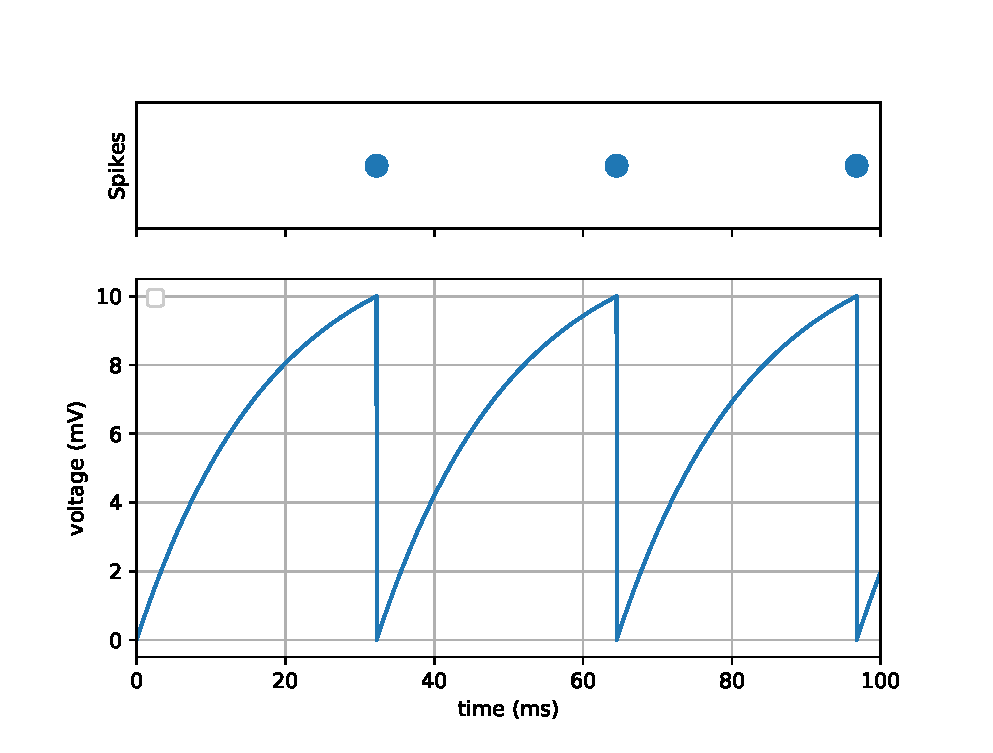
\includegraphics[width=1.0\linewidth]{figures/graphs/singleSpikingNeuron.eps}
        \caption{IF model}
        \label{fig:LIFSingleSpikeGraph}
    \end{subfigure}%
    \begin{subfigure}{.5\textwidth}
        \centering
        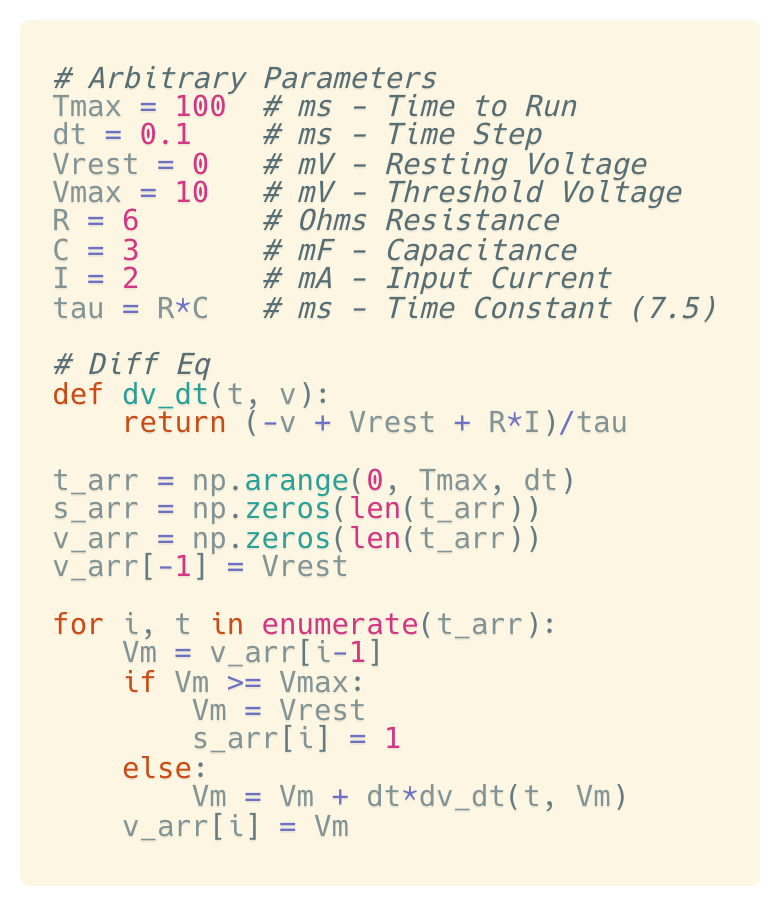
\includegraphics[width=1.0\linewidth]{figures/code/SingleLIFCode.png}
        \caption{IF Python code}
        \label{fig:LIFCode}
    \end{subfigure}
    \caption{Simulation of a single LIF neuron}
    \label{fig:LIFSingleSpikeGraphCode}
\end{figure}

\subsection{Descritization}

Simulating a neuron computationally requires integrating its component
differential equations with respect to time. This can be achieved by defining a
suitably small time-step $dt$ with which to perform descritization. While the
simulation in figure \ref{fig:LIFSingleSpikeGraphCode} above used $dt = 0.1_{ms}$,
this was a fairly arbitrary value and it is worth evaluating the relative
accuracy of different $dt$ values. 

\begin{figure}[h!]
    \centering
    \addtolength{\leftskip} {-3cm}
    \addtolength{\rightskip}{-3cm}
    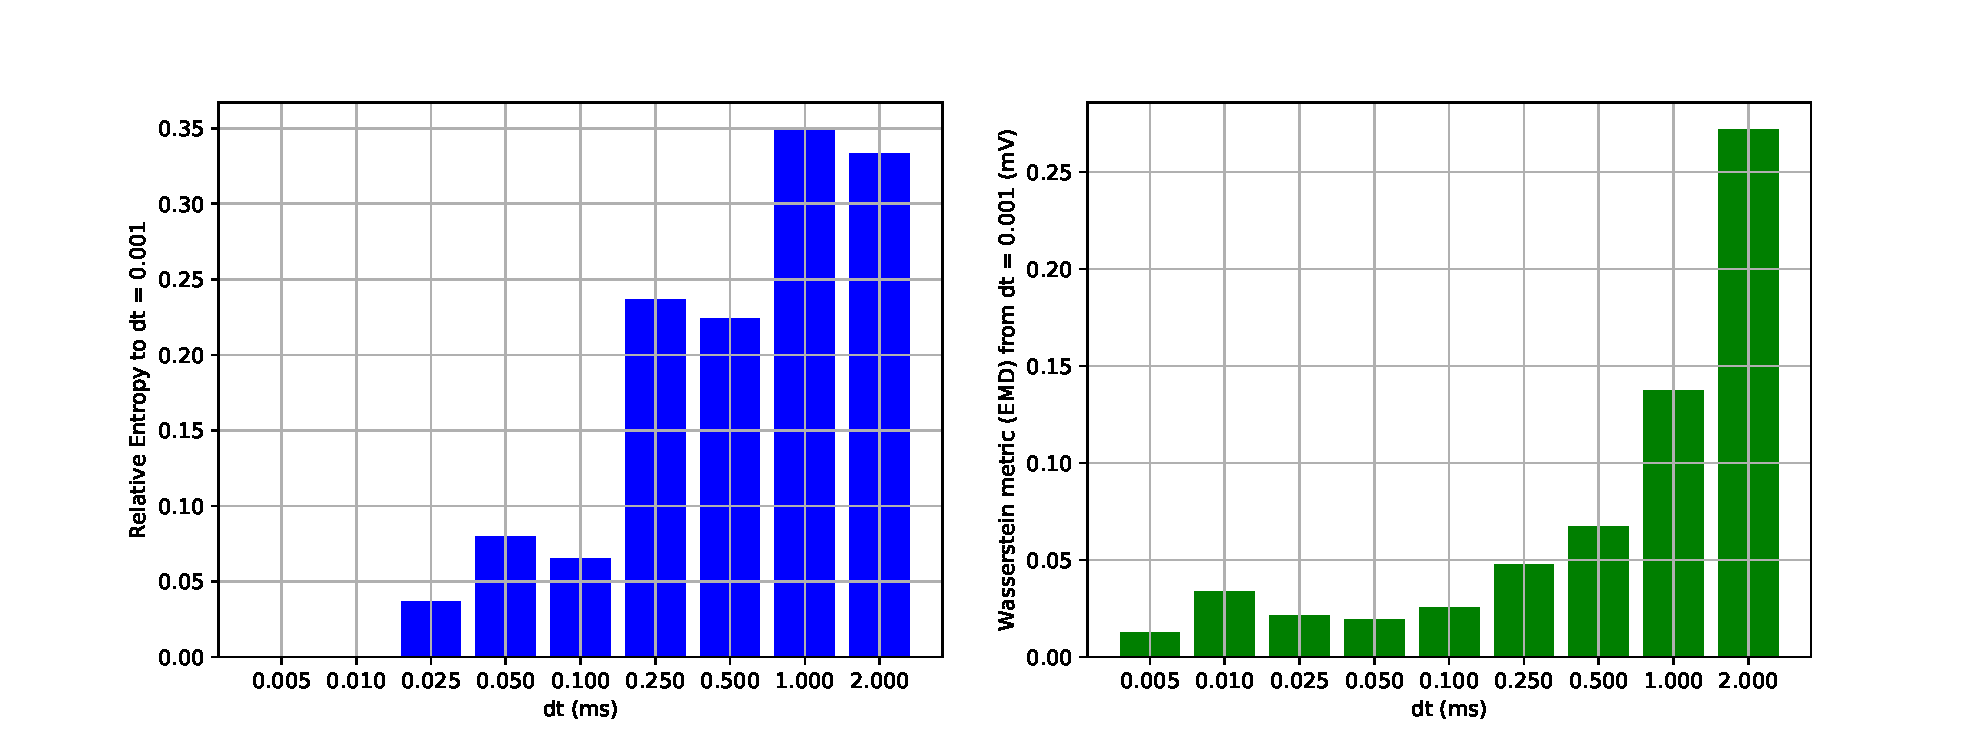
\includegraphics[width=1.4\linewidth]{figures/graphs/entropyofdt.eps}
    \caption{Comparison of $dt$ values, relative to $dt=0.001ms$}
    \label{fig:entropyofdt}
\end{figure}

\FloatBarrier

Figure \ref{fig:entropyofdt} compares the
error produced with different values of $dt$. To
produce this, a distribution $N_{dt}$ of the potential $Vm$ over a single neuron
was created for each value of $dt$, with all other parameters kept equal, and
those distributions compared to the baseline distribution $N_{dt=0.001}$. The
comparison of these distributions was performed by measuring the relative
entropy (Kullback-Leibler divergence) and Earth Movers' Distance between them.
These methods of comparing distributions are described and evaluated in TODO
REF. Increasing the value of $dt$ can be seen to exponentially increase both the
divergence and distance between these distributions, and as such it is clear
that minimising the value of $dt$ is optimal. Computationally it is known that
the error produced from descritization increases by $O(dt)$ for each time
interval \autocite{brette_simulation_2007}.

Using Kullback-Leibler divergence and Earth Movers' Distance to compare potential
distributions is not without drawbacks, and these are discussed in further depth
below.

\subsection{Synapse mechanics}

Synapses between neurons effectively function as a gate, where the current that
passes through the gate decreases exponentially as time passes without any
pre-synaptic spikes. In general this relationship can be approximated by the
equation \ref{eq:Presynaptic1}, where the current across the synapse at a given
time is the product of the conductivity of the synapse channel $g_{syn}$ and the
reversal potential $E_{syn}$. As a simplification in implementation, this
simulation will deal solely with excitatory synapses, so it can be assumed that
$E_{syn} = 0$.

\begin{myequation}\label{eq:Presynaptic1}
    I_{syn}(t) = g_{syn}(t-t^f_{pre}-t_{del})\cdot(v-E_{syn})
\end{myequation}

The complexity of $g_{syn}$ can be different depending on the intent of the
simulation. For this model it is necessary to implement basic synaptic
functionality, in particular, the delay $t_{del}$ between the firing
time of a pre-synaptic neuron $t^f_{pre}$, and the time $t$ at which the channel
conductivity first reacts to the spike, $t^f_{pre} + t_{del} = t$. The conductance of the synaptic channel should
also reduce exponentially after a spike has occurred. A simple formula that
meets these requirements is shown in equation \ref{eq:Presynaptic2}, where only
the most recent pre-synaptic firing time $t^f_{pre}$ is taken into account.
$\tau_s$ is the time constant of the synaptic channel, where a greater value of
$\tau_s$ increases the time taken for the conductivity to slope off. More
complex models may also specify a resistance or charge associated with the
synapse.

\begin{myequation}\label{eq:Presynaptic2}
    g_{syn}(x) =
    \begin{cases}
        0                       & x < 0  \\
        e^{-(\frac{x}{\tau_s})} & x >= 0
    \end{cases}
\end{myequation}

I found, however, that in implementation there were a few quirks to note. As
many pre-synaptic spikes may occur within the firing time of a post synaptic
spike, simply taking into account the latest spike caused inconsistencies in the
input current on the post synaptic neuron. This effect is illustrated in figure
\ref{fig:LIFDUALBUG}, where the potential over the post-synaptic neuron
$Vm_{post}$ drops sharply when the pre-synaptic neuron spikes. This requires a
slight adjustment to equation \ref{eq:Presynaptic1} such that the current
$I_{syn}(t)$ is a function of multiple pre-synaptic spike times. This fix is
present in equation \ref{eq:presynapticfix}.

% \scalebox{1.5}
\begin{equation}\label{eq:presynapticfix}
    \scalebox{1.5}{$
        I_{syn}(t) = \sum_{t^f_{pre}} g_{syn}(t-t^f_{pre}-t_{del})\cdot(v-E_{syn})
    $}\end{equation}
\vspace{1ex}

\begin{figure}[ht]
    \centering
    \includegraphics[width=0.6\linewidth]{figures/graphs/bugZoomed.eps}
    \caption[Graph of a bug in the initial implementation of synaptic channels]{A zoomed-in graph, depicting a bug in the initial implementation of synaptic channels that causes the potential over the post-synaptic neuron (orange) to drop suddenly after a pre-synaptic spike (blue), instead of an expected smooth decrease.}
    \label{fig:LIFDUALBUG}
\end{figure}


% \begin{figure}[h!]
%     \addtolength{\leftskip} {-2.5cm}
%     \addtolength{\rightskip}{-2.5cm}
%     \begin{subfigure}{.65\textwidth}
%         \centering
%         \includegraphics[width=0.6\linewidth]{figures/graphs/bugZoomed.eps}
%         \caption{$t_{del} = 0ms$}
%         \label{fig:LIFDUAL0DEL}
%     \end{subfigure}%
%     \begin{subfigure}{.65\textwidth}
%         \centering
%         \includegraphics[width=0.6\linewidth]{figures/graphs/bugfixzoom.eps}
%         \caption{$t_{del} = 5ms$}
%         \label{fig:LIFDUALBUGDEL}
%     \end{subfigure}
%     \caption{Two neurons in series}
%     \label{fig:LIFDUAL}
% \end{figure}


\subsection{STDP}

The simulation model described so far has been relatively static once
constructed; other than changes in membrane potential, neural parameters are not
changing, nor are the relationships between neurons. However, in biological
networks, neurons adapt their relationships over time in reaction to new
environments or long term changes, in a process called Hebbian Learning
\autocite{trappenberg_fundamentals_2009}. This process can be replicated in a
spiking neural network through adding a vector of weights to each neuron that
determines the relative connection strength of each pre synaptic input. These
weights will change over time according to the observed correlation between
pre-synaptic and post-synaptic spikes, forming Spike-Time Dependent Plasticity
(STDP) \autocite{iakymchuk_simplified_2015}.

The basic form of STDP is simple; given a synaptic weight between neurons,
$w_{ij}$, the weight changes at each time interval by $dw$, a function of
$t^f_{post} - t^f_{pre}$. A function that provides these heuristics is defined
in equation \ref{eq:stdpdw}, where $\delta t$ is typically $t^f_{post} -
t^f_{pre}$. $A^+$ and $A^-$ are constants that, along with $\tau^\pm$ can be
used to adjust the potentiation and depression rates in the synapse.

\begin{myequation}\label{eq:stdpdw}
    dw(\delta t) =
    \begin{cases}
        A^-\cdot e^{(\frac{\delta t}{\tau^-})} & \delta t < 0 \\ 
        A^+\cdot e^{(\frac{\delta t}{\tau^+})} & \delta t > 0 \\
        0                                      & \delta t = 0
    \end{cases}
\end{myequation}

While STDP could be implemented in a sense by defining the new synaptic weight
    as $w_{ij} = w_{ij} + dw$, this is not desirable as unbounded weights will
    eventually tend towards infinity or 0. However simply clamping the weight
    between a maximum and minimum is not a faithful recreation of Hebbian
    Learning either. Ideally, weight changes towards a boundary become "harder"
    to achieve the closer the weight is to the boundary. This can be achieved by
    defining a minimum and maximum weight, and using it to balance the magnitude
    of the weight change, as seen in equation \ref{eq:stdpdelw}.
    

\begin{myequation}\label{eq:stdpdelw}
    \delta w(\delta t) =
    \begin{cases}
        dw(\delta t) \cdot (w_{ijMAX} - w_{ij}) & dw >= 0 \\
        dw(\delta t) \cdot (w_{ij}- w_{ijMIN})  & dw < 0
    \end{cases}
\end{myequation}

One final consideration to be made is the "learning process", that is, how and
when the system determines the correct values for synaptic weights and
stabilises. There are two main approaches, an unsupervised or supervised model.
In a supervised model, the network will process some test inputs with a known
output state, and the system modifies itself by comparison to this correct
state. By contrast, in an unsupervised model the system adjusts weights in
reaction to input data as it arrives, attempting to find a stable equilibrium
where weights shift minimally with each adjustment [TODO CITE SOMETHING]. As the
simulation being designed will use probabilistic noisy inputs with no known
correct network state, an unsupervised weight update model is desirable. In
order to achieve this, synaptic inputs to a given neuron will need to compete
such that the increased potentiation across one synapse decreases the influence
of competing synapses. Without this competitive model, the system is unlikely to
stabilise [TODO CITE]. This can be achieved by dividing each weight by the sum
of all the weights in the input vector of a given neuron. This is shown in
equation \ref{eq:competitive}, where $I_j$ is the input current on post synaptic
neuron $j$, itself the sum of all the weighted and normalised synaptic currents
$I_{ij}$.

\begin{myequation}
    \label{eq:competitive}
    I_j(t) = \sum_{i}\frac{w_{ij} \cdot I_{ij}(t)}{\sum_{i}w_{ij}}
\end{myequation}

